%\documentclass[conference]{IEEEtran}
\documentclass[conference, letterpaper]{IEEEtran}
%\documentclass[letterpaper, 10 pt, twocolumn]{ieeeconf}

\IEEEoverridecommandlockouts
% The preceding line is only needed to identify funding in the first footnote. If that is unneeded, please comment it out.

%\overrideIEEEmargins                                      % Needed to meet printer requirements.

\usepackage{cite}
\usepackage{amsmath,amssymb,amsfonts}
\usepackage{algorithmic}
\usepackage{graphicx}
\usepackage{textcomp}
\usepackage{caption}
\usepackage{subcaption}
\usepackage{multicol}
\usepackage{xcolor}
\usepackage{lipsum}
\usepackage[outdir=./]{epstopdf}



\def\BibTeX{{\rm B\kern-.05em{\sc i\kern-.025em b}\kern-.08em
    T\kern-.1667em\lower.7ex\hbox{E}\kern-.125emX}}


%%%%%%%%%%%%%%%%%%%%%%%%%%%%%%%%%%%%%%%%%%%
 \makeatletter
\DeclareRobustCommand{\volume}{\text{\volumedash}V}
\newcommand{\volumedash}{%
  \makebox[0pt][l]{%
    \ooalign{$V$\cr\raisebox{0.15em}{\kern0.04em--}\cr}%
  }%
}
%%%%%%%%%%%%%%%%%%%%%%%%%%%%%%%%%%%%%%%%%%%%%%



\title{\LARGE \bf
Constrained Model Predictive Control of Variable Buoyancy Device}

\author{Muhammad Umar Masood, Theophilus Kaaya, Zheng Chen$^{*}$
\thanks{*Corresponding author: Zheng Chen, Email: zchen43@central.uh.edu. This work is supported by Texas Commission of Environmental Quality through Subsea Systems Institute Award \#582-15-57593. }% <-this % stops a space
\thanks{M. U. Masood, T. Kaaya, and Z. Chen are with the University of Houston, Mech. Eng. Dept, 4800 Calhoun Rd, Houston TX 77004.
        {\tt\small mmasood8@uh.edu, tskaaya@uh.edu, zchen43@central.uh.edu}}
}


\begin{document}

\maketitle

\thispagestyle{empty}
\pagestyle{empty}

\begin{abstract}
    This paper presents a design and physics-based dynamic model of an underwater depth control device based on buoyancy change. Negative buoyancy is achieved by decreasing the volume while keeping the mass constant, resulting in a higher density. The nonlinearities are discussed in the context of the operation conditions and the practically fulfilled assumptions. With reasonable considerations, the dynamic model is linearized and state-space equations are developed for such a system. The stability of such systems, when subject to constrained control input, is studied.  A Model-based Predictive Control (MPC), which optimizes the control energy and output error with disturbance rejection and considers constrained control input, is then developed. The controller was simulated using MATLAB with a discrete plant model. An experimental setup was also created to test the controller. The developed MPC was then tested experimentally on the hardware which shows the validity of the dynamic model as well.
\end{abstract}

\begin{IEEEkeywords}
    underwater, variable buoyancy engine, depth-control, Model-based Predictive Control
\end{IEEEkeywords}

\section{Introduction}
According to the Ocean Society \cite{OceanSociety}, over 71\% of the Earth's surface is covered by oceans. However, due to the difficulty in accessing these resources, they remain relatively under-utilized. Oceans play a critical role in shaping both short-term weather conditions and long-term climate changes, and they are also a crucial medium for transportation. All the inter-continental communication passes through fiber optics buried in the depths of oceans. Despite all this importance, to date, oceans are just explored 5$\%$ of their total volume \cite{USDepartmentofCommerce2014HowExplored}. We need to explore waters,  for which the research community needs to study unmanned vehicles capable of maneuvering into the narrow spaces under the ocean depths.

Underwater robots, usually referred to as Remotely Operated Vehicles (ROVs), have their major application as an exploration in the depth of oceans and live to monitor resources and ocean life \cite{Kirkwood2002ActiveROV}. The applications of these underwater vehicles are immensely diverse, and they use different types of propulsion systems mostly depending upon the payload capacity required in these applications. Other than the propellers, which are the most energy-consuming way, every submersible requires some sort of Variable Buoyancy Device/Mechanism to change or maintain depth in its operation. Controlled buoyancy is also  an essential and
necessary part of underwater robots that perform
pick-and-place operations. With increased weight, the underwater robot needs to re-adjust the neutral buoyancy state, to stay at one specific depth. Most of the variable buoyancy devices use seawater \cite{Vasiljevic2019,Kobayashi2010} or gases, either generated by some chemical reactions, \cite{Um2011AVehicles,Chen2017AMuscles,yazji2021buoyancy} or releasing and compressing the air \cite{Wood2015AutomatedCrawler}, and some electro-thermal expansion to increase to volume \cite{Hou2020DevelopmentModule}.

For bladder-based systems, where the volume is increased by generating gases using chemical processes, maintaining the pressure of the bladder is still a  research challenge. At higher depths, the hydrostatic pressure decreases the volume of the same amount of gas produced. Um et. al \cite{Um2011InspiredVehicles} introduced a novel electroactive polymer-based buoyancy control, which is very energy-efficient, with the drawback of its slow response \cite{Chen2017AMuscles}. Contrarily, the systems which involve liquid-based bladder (usually water, which has a density similar to seawater) do not face this issue of pressure difference. This means the pressure inside the bladder can be the same as the hydrostatic pressure of the outside seawater.

Among all other underwater ROVs, biomimetic robotic fish are the more developing underwater robots in the new era because of their smaller sizes, energy efficiency, and high maneuverability \cite{Duraisamy2019DesignReview, Liu2022AWing,Xie2021DesignsReview}.  Given the compact and reasonably manageable size of robotic fish, their buoyancy control device should be compact, easy to operate, and fail-safe. A water bladder-based mechanism with a rigid assembly is still the best solution for variable buoyancy in robotic fish. This mechanism has been designed in different ways for the proof-of-concept and has been tested for its buoyancy and depth control \cite{Yu2017}. In \cite{Vasiljevic2019}, presented a depth control based on the feedback from the ambient light sensor, and the pressure sensor. The controller is implemented with a closed-loop pole placement method and constraints on the control input are not considered. In \cite{Kobayashi2010} presented the water-bladder-based variable buoyancy device, but the controller is not developed for regulating or tracking the depth.  A large depth control device was developed by Mahdi et. al \cite{MahdiCHOYEKH2016} which is capable of going in the depth of up to 1000m. The depth control was developed to stabilize the depth in the $\pm 1 m$ range which fulfills the scope of their application. Claus et. al \cite{Claus2012}  developed ballast-based depth control for a glider, which was designed to keep the glider within a certain range of depth, but not to regulate a specific depth. The results showed a depth control within $\pm 1m $ range. A depth controller is developed by Carneiro et. al \cite{Model2023}, and they showed a regulation error of $2cm$, and a maximum overshoot of $30 \%$ was recorded with a settling time of 100s. For the presented application, a comparably faster response with lower steady-state error is required, which is the main focus of this research.

Cylinder-Piston mechanism-based bladders work with a linear actuator and have limited stroke length for operation. Secondly, the applied voltage which correlates to the speed of linear movement also needs to be physically bound as per the design of the linear actuator. These two are hard constraints that really affect the closed-loop performance and stability of the system. If these constraints in the control input and other states are not  considered for, the physical system may go to an unstable state, and some cases can become uncontrollable, especially because of the physical bounds on the control input \cite{Scokaert1998,Rawlings}. For this issue, a more novel and practical approach for depth control in the variable buoyancy engine must be designed and implemented which can take care of the constraints and has disturbance rejection, optimizes the energy, and minimize the tracking error.


This paper presents the physics-based dynamic model of the cylinder-piston mechanism operated in underwater circumstances, and the buoyancy control device (BCD). A fourth-order coupled state space model is developed taking into account the hydrostatic pressure of water and the pressure in the device because of volume change. A methodology to find the model for the cylinder-piston mechanism in an empirical way is also proposed. A Model-based Predictive Control (MPC) is designed considering the combined physics-based and empirical model of the system, and hard constraints on the control input. For the experimental validation, a depth control device is designed. The paper shows the experimental validation of the MPC design, its performance, and hence the dynamic model of the system.


\section{Dynamics and State Space Model}



\subsection{Governing Equation of Buoyancy Control Device}
A dynamic model of the depth control device is developed based on Newton's law of motion. The governing equations were formulated with the free-body diagram. The free-body diagram can be seen in Figure \ref{fig:my_label}, where the position $x$ of the body is shown as the depth in water considering the floating body to be at the equilibrium position of $x=0$. With this reference position, the drag force is upwards, as shown.
\begin{figure}[b!]
    \centering
    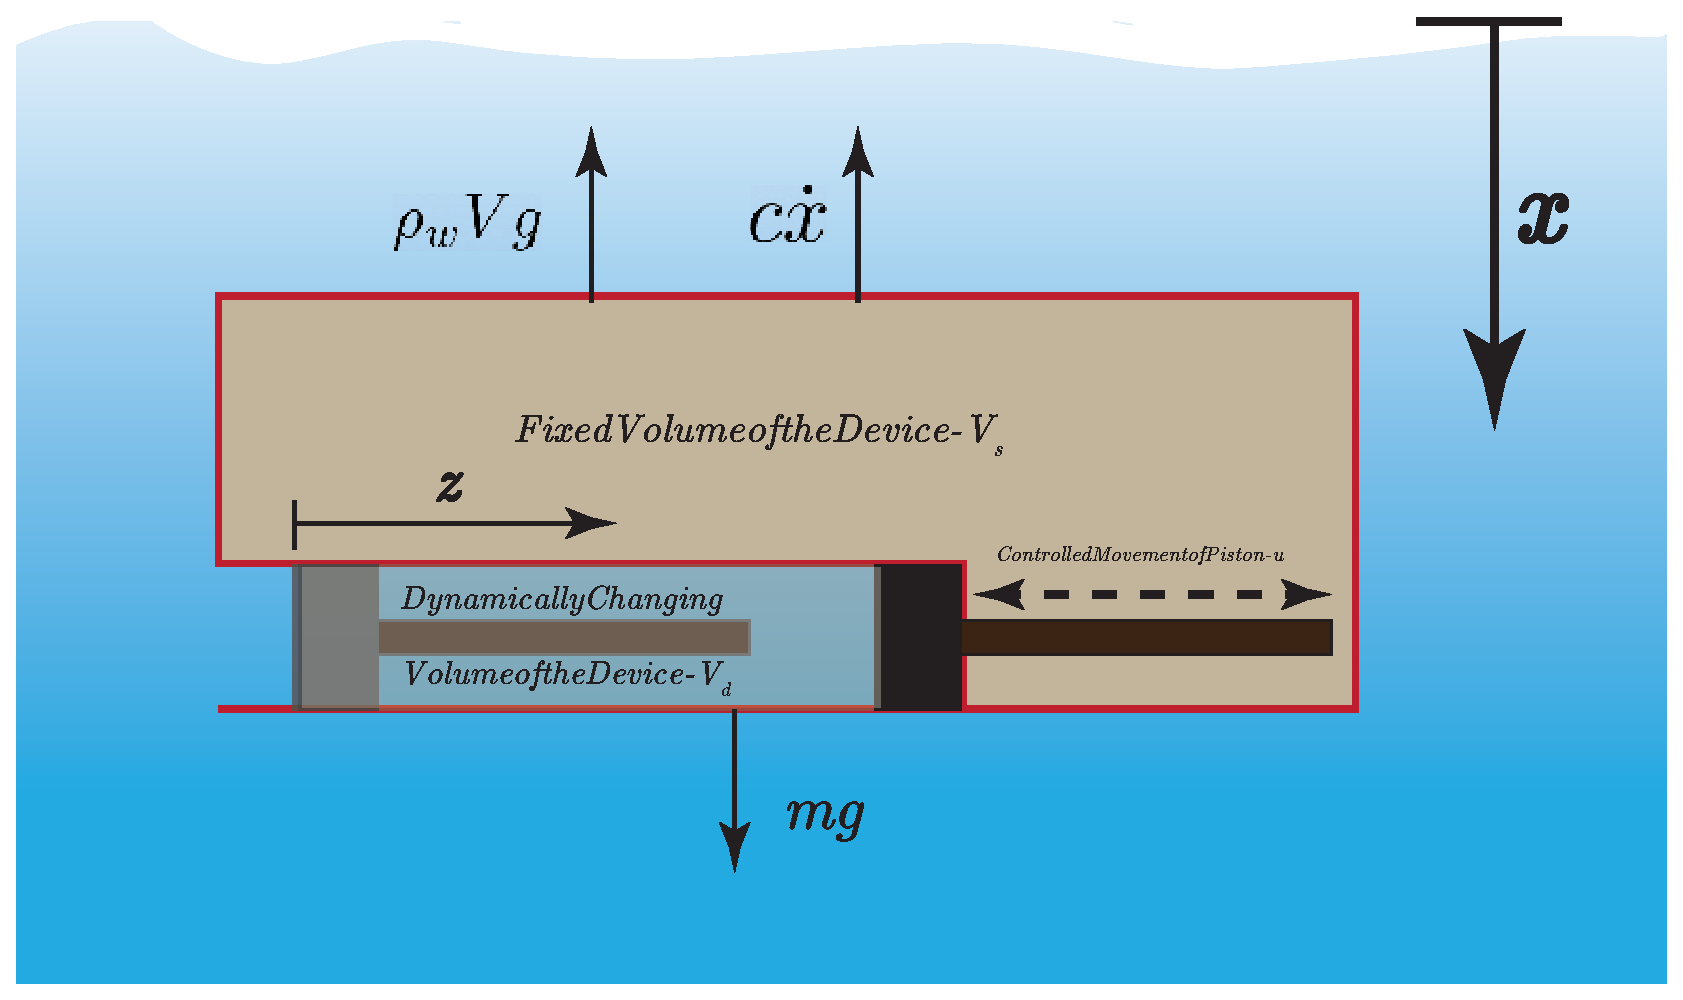
\includegraphics[width=8cm]{images/BCD_Schematic.eps}
    \caption{Free Body Diagram of depth control device.}
    \label{fig:my_label}
\end{figure}

It should be noted at this point that the mass of the device $m$ is constant throughout its operation. With changing position of the piston, the volume of the device is changing which makes it positive or negatively buoyant.   When pulling the cylinder, notated as the positive movement of the piston $z$, the device decreases its volume by $\volume_d$, and when pushing the cylinder out, the device gains an extra volume. The relative density of the device is what relates to the buoyant force.
\begin{equation}
    F_b = -\rho_w (\volume_s + \volume_d) g.
\end{equation}

The fixed or static volume of the device is considered in the state of neutral buoyancy, which means the device is floating and near to being sunk. This condition is more of a theoretically unstable equilibrium point, which is not easily achievable practically. This condition is defined as
\begin{equation}
    \frac{m}{\volume_s} = \rho_w,
    \label{eqn:neub}
\end{equation}
where $\volume_s$ is the fixed volume of the device, having the piston position at zero, and $\rho_w$ is the density of water. The overall volume of the device is hence $\volume = \volume_s - \volume_d$.

Using the free-body diagram shown in Figure \ref{fig:my_label}, Newton's law of motion is described as
\begin{equation}
    % m\Ddot{x} &= \Sigma F  \nonumber \\ 
    m\Ddot{x} = - \rho_w (\volume_s + \volume_d) g - c_d\dot{x} + mg,
\end{equation}
where $\volume_d$ is the dynamic portion of the volume which can be controlled through the position of the piston in the cylinder. $g$ is the acceleration due to gravity, and $c_d$ is the drag coefficient of the device. Substituting for $\volume_s$ and $\rho_w$, the second-order Ordinary Differential Equation (ODE) can be simplified to
\begin{equation}
    \Ddot{x} + \frac{c_d}{m}\Dot{x} = \frac{g}{\volume_s}\volume_d.
    \label{eqn:device_eom}
\end{equation}
The right-hand side of the equation is the external driving force of the system. $\frac{g}{\volume_s}$ is constant and the control is %$\volume_d$.
The piston movement in the cylinder is shown in Figure \ref{fig:cyl},
\begin{figure}[b!]
    \centering
    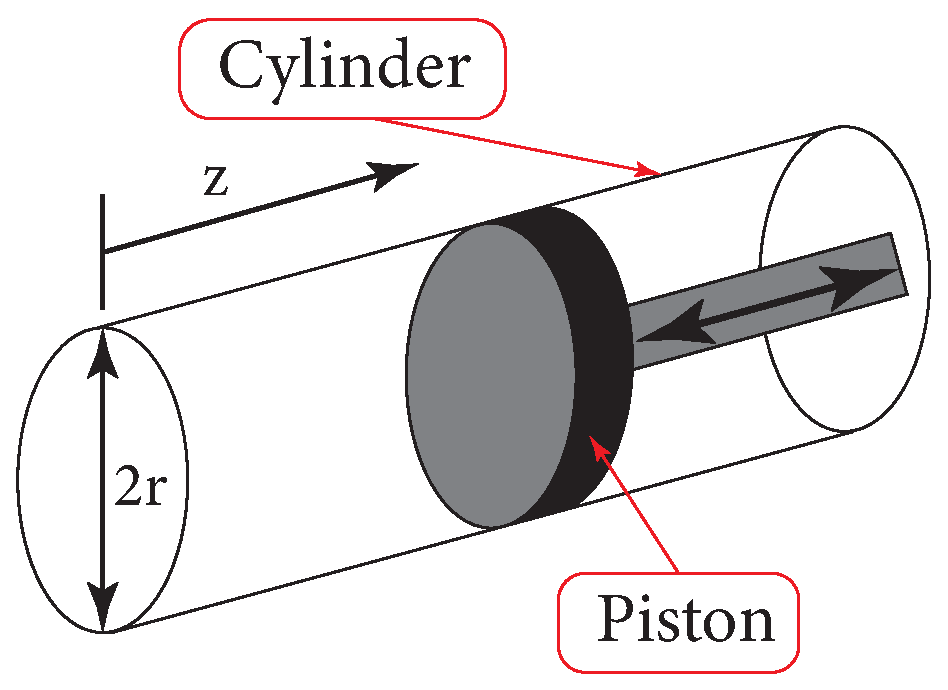
\includegraphics[width = 4cm]{images/Cylinder_BCD.eps}
    \caption{Piston movement notations.}
    \label{fig:cyl}
\end{figure}
where $z$ is the position of the piston with the reference shown.
$\volume_d = \pi r_p^2 z$, therefore Equation \ref{eqn:device_eom} becomes
\begin{equation}
    \Ddot{x} + \frac{c_d}{m}\Dot{x} = \frac{g\pi r^2}{\volume_s} z.
    \label{BCD_dynamics}
\end{equation}
This gives a second-order Equation of Motion for the Buoyancy Control Device considering the position of the piston $z$ as the control input to the system.



\subsection{Dynamics of the Cylinder-Piston}
In this section, the dynamics of the cylinder piston are evaluated as an intermediate measure to integrate the actuator dynamics into the model. As mentioned before, the piston movement in the cylinder is achieved by a linear actuator. There are multiple non-linearities and load disturbances involved in the actuation process of the piston. These include:

\begin{enumerate}
    \item An inwards force exerted on the piston/actuator due to the water pressure in depth ($\rho_w g x$) where $x$ is the depth taken from the surface of the water.
    \item An opposing force on the piston caused by the pressure inside the device due to the volume change. Consider the device is air-tight at some pressure $P_s$, which will change when the device volume changes, as per isothermal condition, $PV ={\rm constant}$.
    \item Backlash and dead-zone from the Linear Actuator and its assembly during operation.
    \item Hysteresis during the piston operation. One source of the hysteresis is the shape of the piston rubber causing it to have more friction when sliding in one direction than in another. Another form of hysteresis is due to the nature of the thread force demanding more torque in one direction than the other.
\end{enumerate}

\vspace{10pt}


\subsubsection{Empirical Model of the Linear Actuator}
For the sake of the operation of the actuator, a PD controller is applied to the linear actuator to overcome the non-linearities. The closed-loop response is recorded under certain conditions of interest. These conditions are where the device is actually initially installed. The conditions are as follows:

\begin{enumerate}
    \item The device is air-tight at atmospheric pressure.
    \item The position of the piston $z$ is kept at zero as per the notation used. At the zero position of the piston, the device is neutrally buoyant.
    \item Step response data is collected when the Cylinder-Piston runs underwater at a constant depth of $50 mm$.
    \item To avoid any possible interference from the surroundings, no harness is used for power or data transmission.
\end{enumerate}

Step response of the closed-loop actuator is recorded in the time domain as shown in Figure \ref{fig:PD_cl}.
\begin{figure}[tbp!]
    \centering
    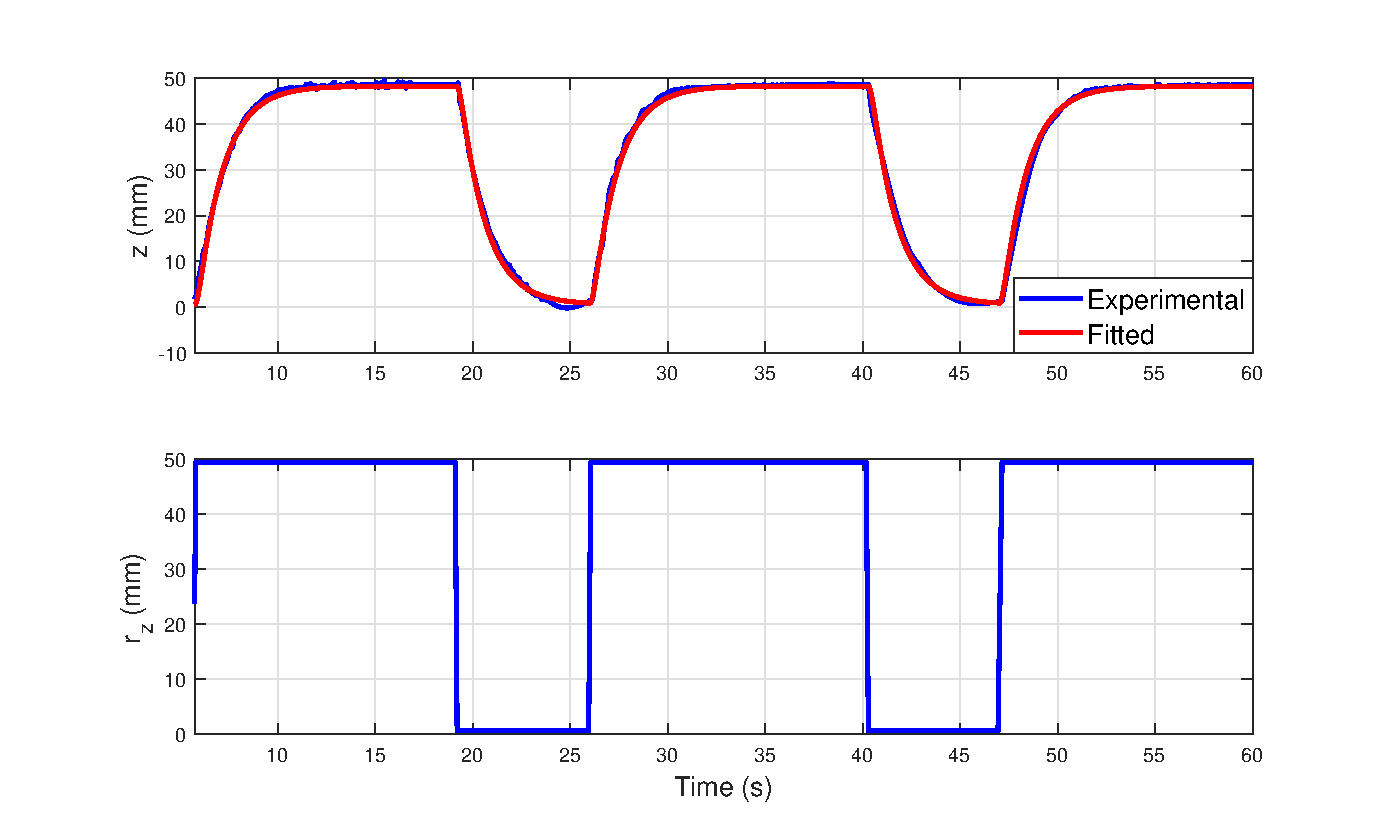
\includegraphics[width = .45\textwidth]{images/PD_CL.eps}
    \caption{Step response of the close-loop linear actuator.}
    \label{fig:PD_cl}
\end{figure}
Linear actuator dynamics are second order so, the second-order transfer function is estimated using a frequency response function to a step input reference of the piston. The second-order approximation gives a good fit to the response data and thus the empirical model is used for the closed-loop sub-system consisting of a PD controller, linear actuator, gearbox, leadscrew, and load disturbances.  The estimated transfer function is
\begin{equation}
    \frac{Z(s)}{R_z(s)} = \frac{4.3171}{(s+5.75)(s+0.7695)}.
    \label{eqn:cltf}
\end{equation}
This closed-loop sub-system is also shown in Figure \ref{fig:controldiag}, where $r_z$ is the reference input for the piston position.


\begin{figure*}[htbp!]
    \centering
    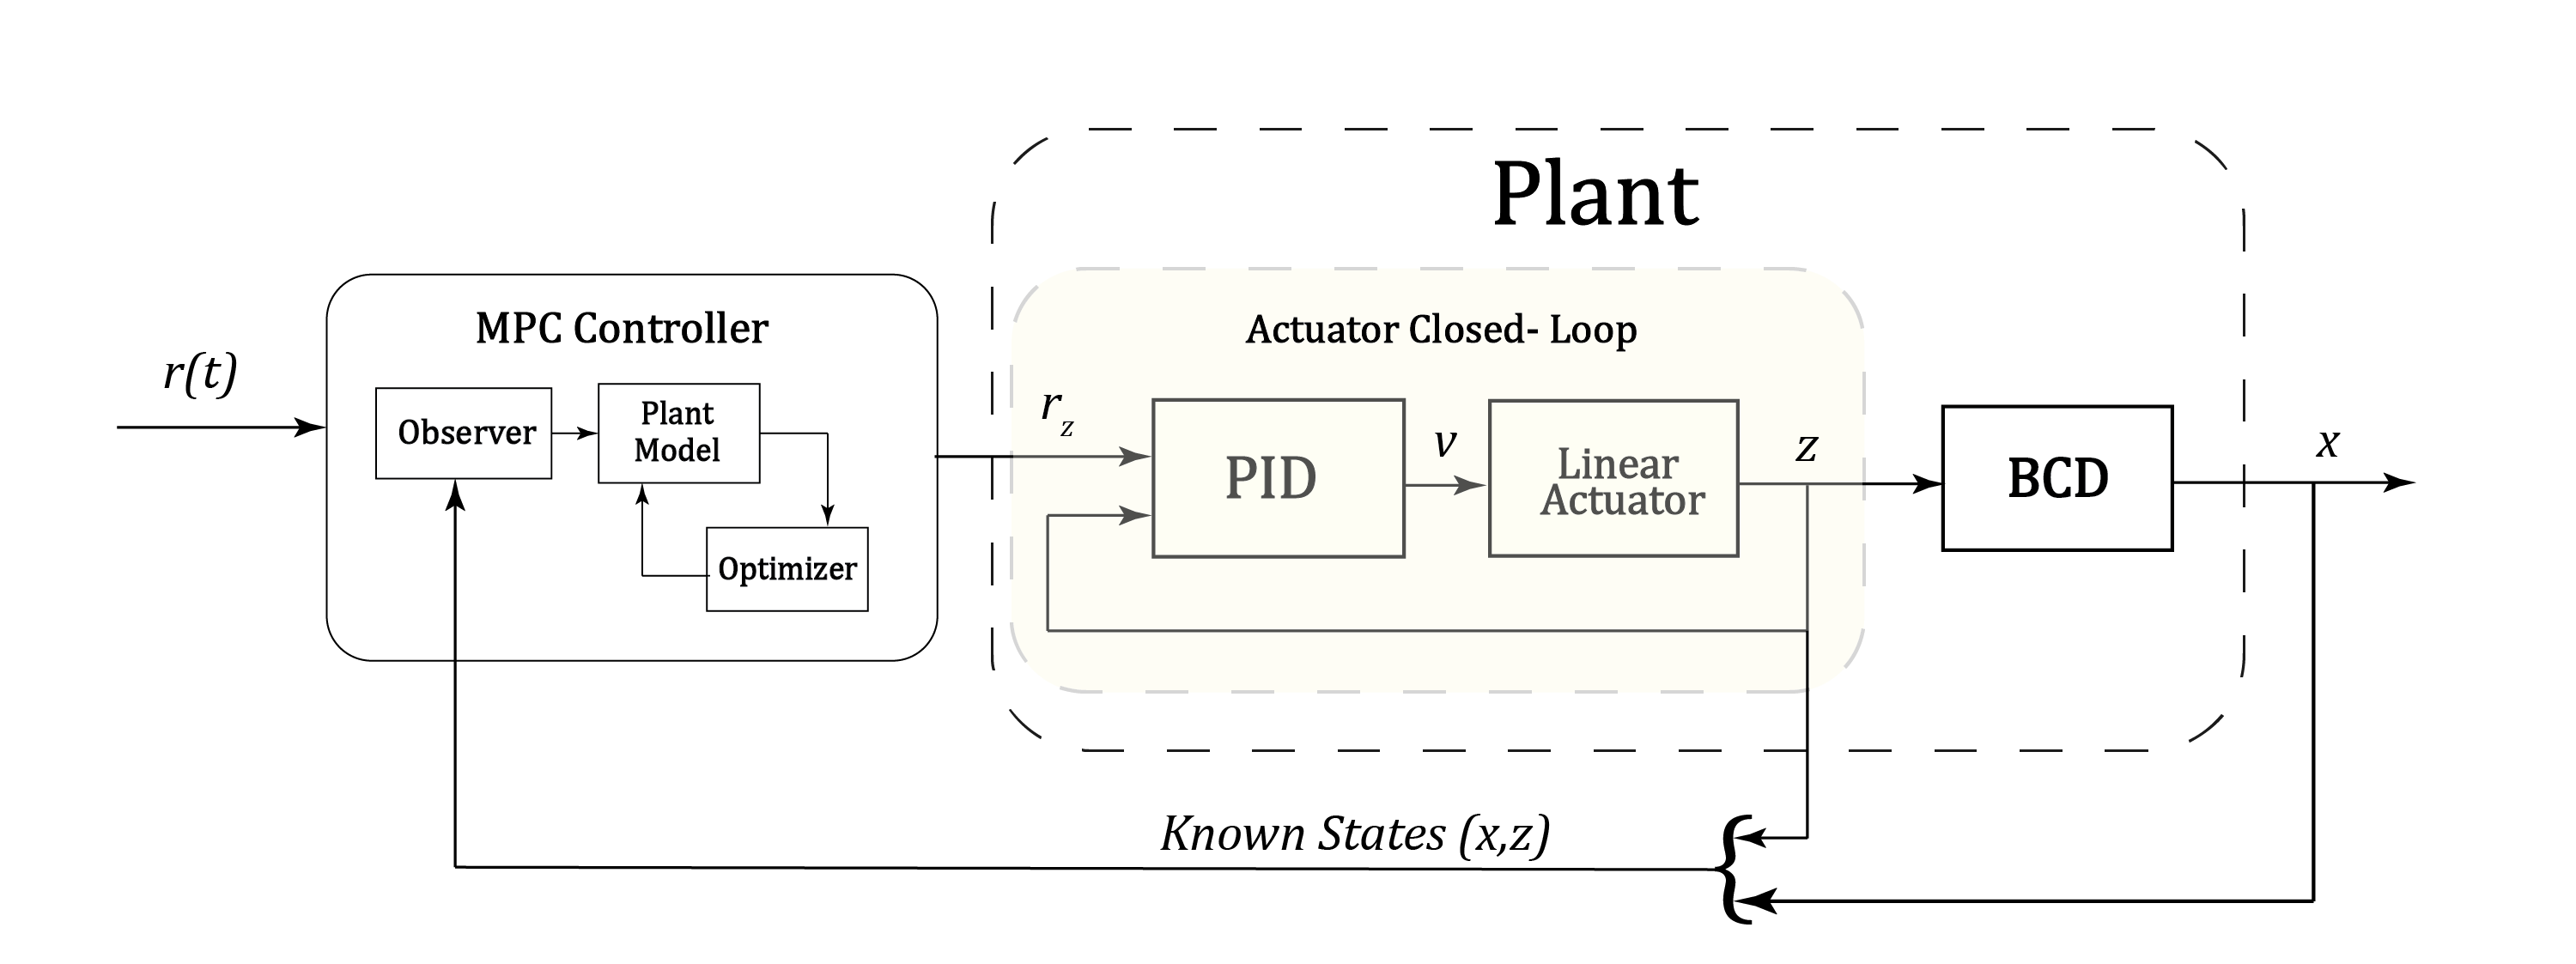
\includegraphics[width = 0.8\textwidth]{images/Control Diagram-01.png}
    \caption{Schematic of the Plant and the MPC Control.}
    \label{fig:controldiag}
\end{figure*}


%%%%%%%%%%%%%%%%%%%%%%%%%%%%%%%%%%%%%%%%%%%%%%%%%%%%%%%%%%
\subsection{State Space Model}\label{sec:state_space_model}

The state space vector for the dynamic model of the complete system is taken as
$
    \mathbf{x} =
    \begin{bmatrix}
        x_1 & x_2 & x_3 & x_4
    \end{bmatrix}^T,
$
where $x_1 = x$, $x_2 = \Dot{x}$, $x_3 = z$, and $x_4 = \Dot{z}$. 

Now the state space representation for the BCD can be written utilitzing the equation of motion as given in \eqref{BCD_dynamics}  and given below in \eqref{eqn:ss_BCD}.
\begin{equation}
    \Dot{
        \begin{bmatrix}
            x_1 \\
            x_2
        \end{bmatrix}
    } =
    \begin{bmatrix}
        0 & 1              \\
        0 & -\frac{c_d}{m}
    \end{bmatrix}
    \begin{bmatrix}
        x_1 \\
        x_2
    \end{bmatrix}
    +
    \begin{bmatrix}
        0 \\
        \frac{g\pi r^2}{\volume_s}
    \end{bmatrix} z
    \\
    \label{eqn:ss_BCD}
\end{equation}

Note that in this equation,  $z$ is the piston position, and the states $x_1$ and $x_2$ are the position and velocity of the BCD, as defined in \eqref{BCD_dynamics}.
\\

The closed-loop transfer fucntion of the piston actuator is defined emperically in \eqref{eqn:cltf}, which can be written in state space representation as follows


\begin{equation}
    \Dot{
        \begin{bmatrix}
            x_3 \\
            x_4
        \end{bmatrix}
    } =
    \begin{bmatrix}
        0     & 1     \\
        -4.43 & -6.52
    \end{bmatrix}
    \begin{bmatrix}

        x_3 \\
        x_4
    \end{bmatrix}
    +
    \begin{bmatrix}

        0 \\
        4.32
    \end{bmatrix} r_z.
    \\
    \label{eqn:ss_cl_act}
\end{equation}
Now combining the both second orders subsystems (1) BCD and (2) closed-loop linear actuator model, the state space representation of the cascaded 4th order system becomes



\begin{multline}
    \Dot{
        \begin{bmatrix}
            x_1 \\
            x_2 \\
            x_3 \\
            x_4
        \end{bmatrix}
    } =
    \begin{bmatrix}
        0 & 1              & 0                          & 0     \\
        0 & -\frac{c_d}{m} & \frac{g\pi r^2}{\volume_s} & 0     \\
        0 & 0              & 0                          & 1     \\
        0 & 0              & -4.43                      & -6.52
    \end{bmatrix}
    \begin{bmatrix}
        x_1 \\
        x_2 \\
        x_3 \\
        x_4
    \end{bmatrix}
    +
    \begin{bmatrix}
        0 \\
        0 \\
        0 \\
        4.32
    \end{bmatrix} r_z.
    \label{eqn:ss_empirical}
\end{multline}

The output is defined as the position of the BCD in depth
\begin{equation}
    y =
    \begin{bmatrix}
        1 & 0 & 0 & 0
    \end{bmatrix} \mathbf{x}
\end{equation}

\subsubsection*{System Analysis}
Considering Equation \ref{eqn:ss_empirical}, there is at least one eigenvalue of the A matrix which is $0$ so the system is unstable. This accounts for why the equilibrium point (floating in neutral buoyancy) is unstable. The controllability and observability matrices are full-rank, so the system is fully controllable and observable.





\section{Model-based Predictive Control (MPC)}
MPC is an optimal control technique that calculates control inputs dynamically while minimizing a cost function/performance index on a finite horizon length $T$ at a point in time $t_0$ \cite{Rawlings}. The performance index is chosen to be linear quadratic of the form
\begin{equation}
    \begin{aligned}
        J(t_0)= \sum_{t_0}^{T+t_0}{{((C\mathbf{x}-r)}^TQ(C\mathbf{x}-r)+\mathbf{u}^TR\mathbf{u})dT},
    \end{aligned}
    \label{eqn:J}
\end{equation}
where, $Q$ is the tracking weight and $R$ is the control input weight, with the conditions  $ Q\succ0, R\succ0$, and $r$ is the tracking reference signal. For the regulator problem, $r$ can be zero or a constant. The time period for which the cost function is defined as the prediction horizon, in this case, $[t_0 \; T+t_0$. In the controller design on BCD, the prediction horizon is set to 80 steps. This performance index in \ref{eqn:J} is minimized, and on the optimal value of the performance index, the control input is calculated, considering the hard constraints on the control input signal,
\begin{equation}
    |u| < u_b,
\end{equation}
where $u_b$ is the bounded input, which means the maximum control input value that can be achieved physically. For the piston in the described system, $u_b = 20$ mm.

Linear Quadratic MPC is designed and implemented using the MATLAB Model Predictive Toolbox \cite{mathworks_MPC}, which after solving the Algebraic Ricatti Equation (ARE) numerically, calculates the linear control law gain $K_c$ for the span of control horizon $[t_0 \; T_c+t_0]$.
\begin{equation}
    u=-K_c\mathbf{x}.
\end{equation}
In the designed controller, the control horizon is set to 20. After each control step is applied to the system, the MPC model is run again on the shifted prediction horizon of $[t_0+1 \; T+t_0+1]$.
Using the depth sensor, one state which is also the output of the system, is directly measured. Based on the output feedback, using an internal observer, the MPC estimates the other three states and forms the full-state feedback $\mathbf{x}$ which is required for the cost function.



\subsection{Controller Design and Simulation}
For the controller design in MATLAB, the plant is discretized for a sampling time of 0.1 s and the penalty weights for the output error and control input are set to $Q = 1$ and $R = 40$ respectively. All the parameters used for the simulation and experiments are listed down in Table \ref{tab1}. The performance of the MPC controller is simulated using the dynamic model \ref{eqn:ss_empirical} described in the previous section \ref{sec:state_space_model}, and shown in Figure \ref{fig:sim_80mm_unsat}.
\begin{figure}[t!]
    \centering
    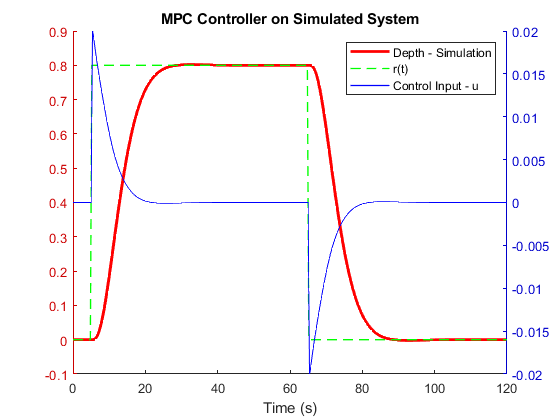
\includegraphics[width = 0.45\textwidth]{images/Simulation - Tracking 80mm - Unsaturated - 1-40.png}
    \caption{Simulated Response of the BCD for $R = 40$ and $Q = 1$.}
    \label{fig:sim_80mm_unsat}
\end{figure}
In this example, the penalty weight for the control input is set high so the optimization algorithm calculates lower control input by trading off the response time of the output. It is important to note here that the system could still go faster than this response because the full control input is not utilized.

%For faster response, $R = 20$ is used. It can be observed in Figure \ref{fig:sim_80mm_sat}
%\begin{figure}[htbp!]
%    \centering
%    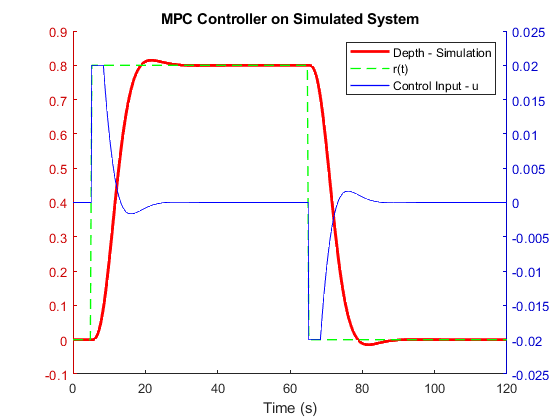
\includegraphics[width = 0.42\textwidth]{images/Simulation - Tracking 80mm - Saturated - 1-20.png}
%    \caption{Simulated Response of the BCD with Saturation in control input for $R = 20$ and $Q = 1$}
%    \label{fig:sim_80mm_sat}
%\end{figure}
%that the control input is now higher and saturates to its maximum physical limit set in the MPC controller. The MPC controller does not generate any higher inputs than the constraints defined above. Since this is a closed-loop system with MPC knowing the future control values, the saturated input is not held for a long time preventing the system from going out of the stability envelope. Faster response can be achieved by further reducing the control effort weight, $R$ in the cost function \ref{eqn:J} , as shown in Figure. \ref{fig:sim_80mm_sath}.
%\begin{figure}[htbp!]
%   \centering
%    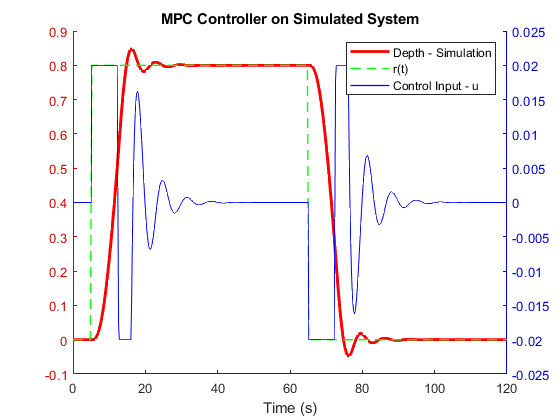
\includegraphics[width = 0.48\textwidth]{images/Simulation - Tracking 80mm - Saturated - 1-1.png}
%    \caption{Simulated Response of the BCD with the saturation of control input for $R = 1$ and $Q = 1$}
%    \label{fig:sim_80mm_sath}
%\end{figure}



\section{Experimental Validation}
A depth control device is developed for the experimental testing of the proposed model and Linear Quadratic Model Predictive Controller. A cylindrical-shaped enclosure of the device is designed to achieve IP67 standard liquid immersion safety,  using O-ring vacuum face sealing with 10\% compression ratio. Small buckets are designed in the bottom portion for the dead weights, to adjust the mass of the device and the weight-balancing, so that it is neutrally buoyant with no control input. The buckets are designed in such a way that the center of mass can also be adjusted by varying the mass distribution in different buckets. The enclosure is fabricated using \texttrademark Form Labs Form 3 Stereolithography (SLA)\cite{formlabs} printer using Clear Resin material. The experimental Setup and the Depth Control Device are shown in Figure. \ref{fig:dcd_hardware}

A cylinder and piston mechanism is also designed and fabricated, which is water-proof. The piston is actuated using Actuonix Motion Devices L12 miniature linear actuator with a translational-potentiometer feedback\cite{L12}. The depth control device is shown in  Figure \ref{fig:dcd_hardware}.
\begin{figure}[b]
    \centering
    \begin{subfigure}[h]{0.2\textwidth}
        \centering
        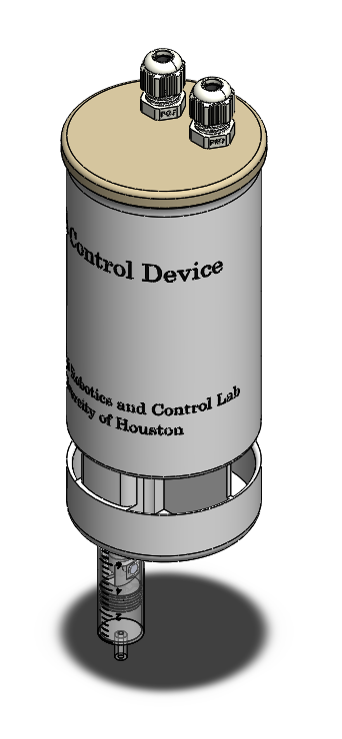
\includegraphics[height=6cm]{images/DCD_hardware.png}

    \end{subfigure}%
    \begin{subfigure}[h]{0.2\textwidth}
        \centering
        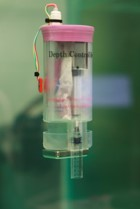
\includegraphics[height=6cm]{Picture1.jpg}

    \end{subfigure}
    \caption{CAD model and the fabricated depth control device.}
    \label{fig:dcd_hardware}
\end{figure}

%\begin{figure}[htbp!]
%    \centering
%    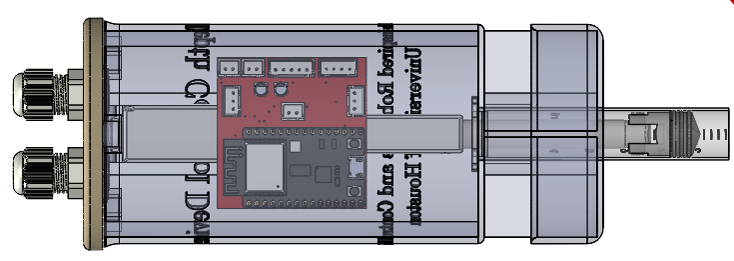
\includegraphics[width = 0.35\textwidth]{images/DCD_hardware3.png}
%   \caption{Transparent View of the DCD}
%   \label{fig:dcd_tr}
%\end{figure}

The power source, application-level microcontroller, and driving circuitry are all self-contained within the device to avoid any disturbances because of the harness. The ESP32C3 microcontroller from Espressif Systems\texttrademark \cite{esp32_c3} is used along with the motor driver IC from  Texas Instruments\texttrademark for the onboard operation of the linear actuator. A Water Pressure Sensor LPS33 from  STMicroelectronics\texttrademark is used for the depth feedback. Wireless communication using UDP protocol via $IEEE 802.11n$ is established between the device and the host computer running MATLAB 2022b.

The device sends the updated  sensor data to the computer, MPC in MATLAB implements the Kalman Estimator and the state observer registers it as full-state feedback. Based on the full-state feedback, the MPC calculates the control input, which is then communicated back to the onboard controller, wirelessly. The sampling time in the discretization of the plant model and MPC design is consistently set as 0.1 s, so a synchronous communication is set up between the computer and the device with a fixed time step of 0.1 s.  Other parameters of MPC are used the same as for simulations, listed in Table. \ref{tab1}. The experimental setup is shown in Figure \ref{fig:es}.

\begin{figure}
    \centering
    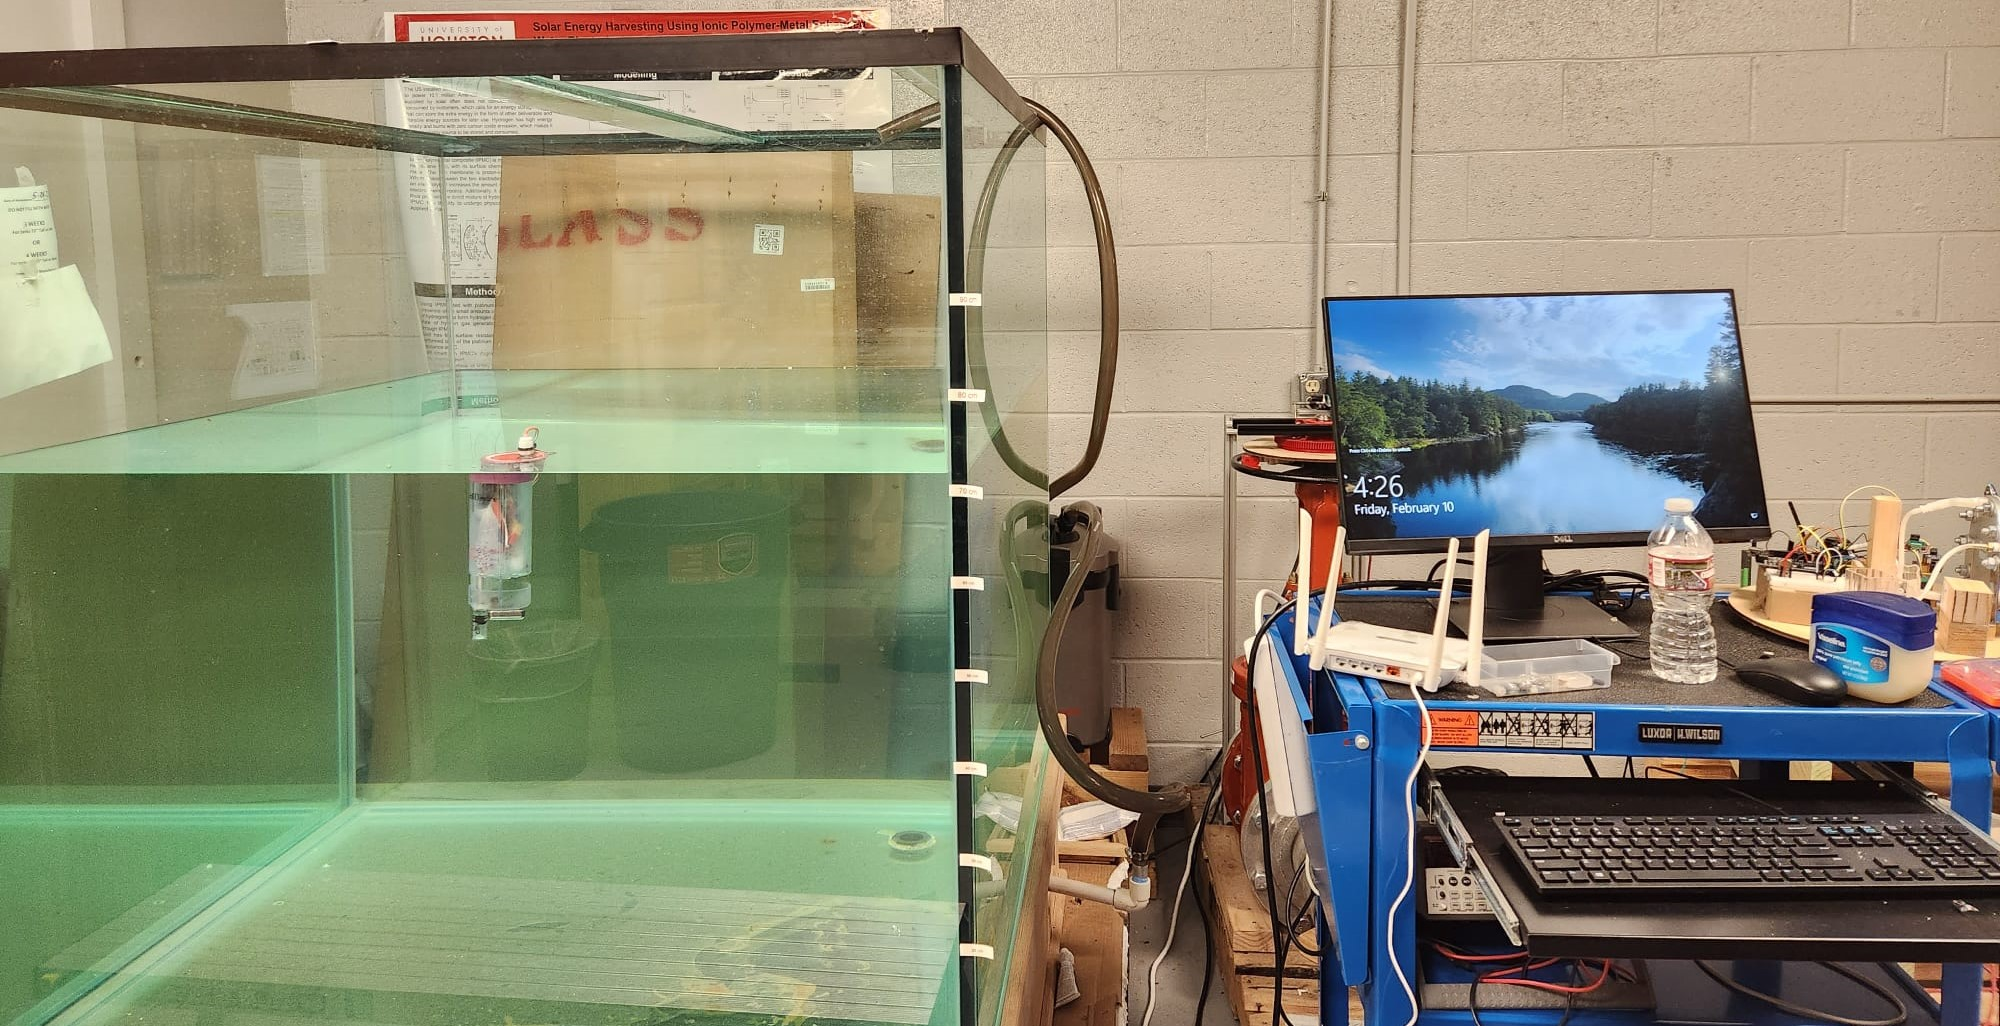
\includegraphics[width = 0.45\textwidth]{Experiment Setup.jpg}
    \caption{Experimental setup.}
    \label{fig:es}
\end{figure}

\begin{table}[b]
    \caption{Parameters for Simulation and Experiment}
    \begin{center}
        \begin{tabular}{|c|c|c|c|}
            \hline

            \textbf{Parameter}       & \textbf{Symbol} & \textbf{Value} & \textbf{Units} \\
            \hline
            Sampling Time            & $t_s$           & 0.1            & $s$            \\

            \hline
            Prediction Horizon       & $T$             & 80             & $steps$        \\
            \hline
            Control Horizon          & $T_c$           & 20             & $steps$        \\
            \hline
            Constraints for Actuator & $u_b$           & 20             & $mm$           \\
            \hline
            Damping Coefficient      & $c$             & 0.192          & $Nms^1$        \\

            \hline
            Mass                     & $m_d$           & 0.683          & $kg$           \\

            \hline
        \end{tabular}
        \label{tab1}
    \end{center}
\end{table}

To record the data following considerations are practically taken care of:
\begin{enumerate}
    \item When the enclosure is closed, the piston position is set to zero.
    \item Ensured that the enclosure/device is perfectly air-tight for the range of operation. To ensure this, the device is kept underwater at a certain depth of interest (in this case $50$ cm) for three times more duration of the experiment time (in this case three minutes) and checked for any immersion of water.
    \item The device is set to neutrally buoyant, by manually adjusting the dead weights.
    \item The weight distribution in the device is such that the device will always stay in the vertical orientation.

\end{enumerate}

The experiment is performed for a step input of $35$ mm and the depth response is shown in Figure \ref{fig:exp_step}
\begin{figure}[bp!]
    \centering
    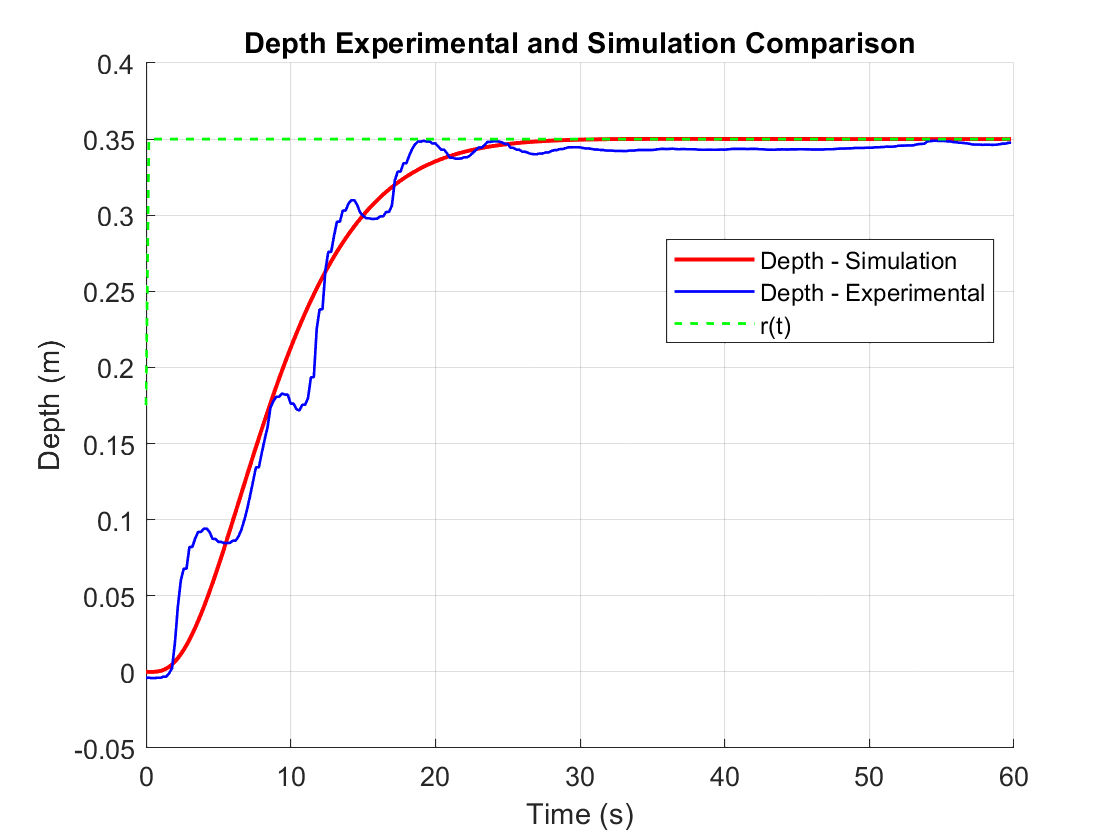
\includegraphics[width = 0.5\textwidth]{Exp_Result.png}
    \caption{Comparison of the simulated plant output and experimental results.}
    \label{fig:exp_step}
\end{figure}
as a comparison to the simulated output on the modeled plant in MATLAB. The response shows that the proposed controller has good steady-state performance which is one important parameter for small underwater robots like biomimetic robotic fish. Maintaining a certain depth is required for most underwater missions like tracking pipelines and for monitoring and performing pick-and-place operations. The transient response, however, has some sort of vibrations due to non-linearities in the physical system which may not have been catered for in the dynamic model used in the MPC. The results show that MPC can provide acceptable rejection to the unmodeled disturbances.


\section{Conclusion}
A new and more practical dynamic modeling approach for a Cylinder-piston type bladder based/volume-changing depth control device is proposed, which is the backbone of any biomimetic underwater robotic fish or remotely operated vehicles (ROVs). The dynamic model of the mechanism is presented based on the physics of the system. A simplified yet accurate empirical way is proposed for the complex dynamics of the piston movement. A linear state-space representation is formed which is a very handy tool for analyzing the system's behavior in terms of stability, controllability, and observability.
An MPC-based controller is designed and implemented on the device and tested for regulation and tracking. Steady-state tracking performance is found to be within 2 percent error bounds, which provides enough stability that this system can be used in underwater surveillance robots.
The control range is experienced to be very limited and depends on the size of the cylinder. A 10-milliliter cylinder has a considerably faster response as shown in the experimental results. Pick and place or interactive tasks are some main applications in underwater robotics. This range of volume change is surely not enough for these applications. In the future, this method can be combined with an ionic polymer-metal composite (IPMC) based solution which has a theoretically unlimited range of buoyancy change. The biggest challenge in IPMC-based solution is the slow response which can be catered for with the presented approach.

\section*{Acknowledgment}

This research is supported by Texas Commission on Environmental Quality through Subsea Systems Institute Award \#582-15-57593.  This project was paid for [in part] with federal funding from the Department of the Treasury through the State of Texas under the Resources and Ecosystems Sustainability, Tourist Opportunities, and Revived Economies of the Gulf Coast States Act of 2012 (RESTORE Act).  The content, statements, findings, opinions, conclusions, and recommendations are those of the author(s) and do not necessarily reflect the views of the State of Texas or the Treasury.

\bibliographystyle{ieeetran}
\bibliography{IEEEabrv,references}

\end{document}
